\documentclass[16pt,a4paper]{article}

\usepackage{fontspec}
\setmainfont[BoldFont=黑体]{宋体}          
\XeTeXlinebreaklocale "zh"                    
\XeTeXlinebreakskip = 0pt plus 1pt minus 0.1pt  

\usepackage{indentfirst} 
\setlength{\parindent}{2em}

\usepackage{changepage}
\usepackage{float}
\usepackage{setspace}
\usepackage{amsmath}
\usepackage{amsfonts}
\usepackage{amssymb}
\usepackage[colorlinks,linkcolor=black,anchorcolor=black,citecolor=black]{hyperref}

\usepackage{geometry}
\geometry{left=2.5cm,right=2.5cm,top=2.5cm,bottom=4cm}
\usepackage{fancyhdr}
\pagestyle{fancy}
\lhead{\includegraphics[scale=0.5]{logo.png}}

\author{郭嘉丞 \quad 姚皓天}
\title{数字听诊器 \\ Digital Stethoscope}
\date{2015年6月}

\graphicspath{{Figure/}}

\begin{document}
\maketitle
\thispagestyle{empty}
\newpage
\section{简介}
\subsection{设计目的}
听诊器是一种常用的医疗设备,在初步诊断中有重要的作用。传统的听诊器对于人体内部的声音型号是一个固定的低通系统,具有很高的信噪比但是通带与放大倍数都不可调。同时也不能够记录听到的声音用于回放进行详细诊断以及教学。针对这些问题,电子听诊器被设计出来进行放大,滤波与录音。\linebreak
在本次课程设计中我们自己搭建了一个电子听诊器。完成硬件设计、调试以及软件编程的工作。
\subsection{基本功能}
\begin{enumerate}
\item 能够采集到人体内部的声音信号进行放大与回放
\item 能够存储听诊器中听到的声音
\end{enumerate}

\subsection{可以拓展的功能}
\begin{enumerate}
\item 提供不同的滤波模式用于不同种声音的采集
\item 实现心跳次数的自动测量
\item 能够实现在呼吸音和心跳音混合的情况下提取并放大较弱的呼吸音。
\end{enumerate}
这些功能由于时间所限没有完成,其中不同滤波模式可以考虑增加可调滤波电路或者使用数字滤波器完成,而之后的两个功能主要是信号处理的内容,与模拟电子部分关系不大。

\section{系统设计}
\begin{figure}[H]
\centering
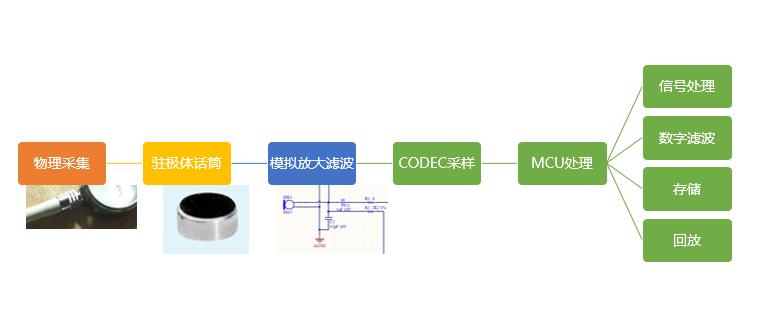
\includegraphics[scale=0.8]{system.png}
\caption{系统总体框图}
\end{figure}
\begin{figure}[H]
\centering
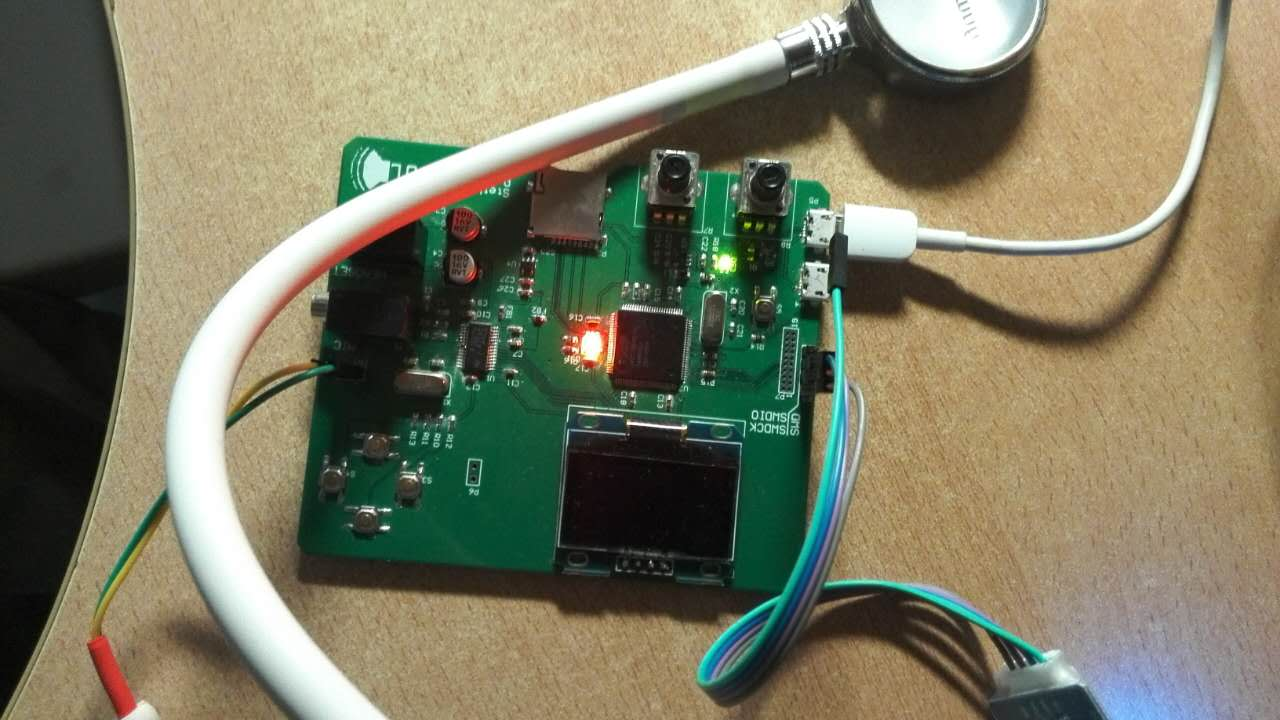
\includegraphics[scale=0.3]{board.jpg}
\caption{实际产品图片}
\end{figure}
物理采集系统直接使用了购买的听诊器中的听筒与导管,放入驻极体话筒后密封。导管本身就带有了物理放大的功能。之后对驻极体话筒采集到的信号使用共源放大电路进行放大。之后使用专用音频CODEC进行采样以及模拟输出,也就是ADC/DAC。对于已经数字化的信号使用微控制器NXP1768进行处理,可以进行保存,回放,滤波等信号处理工作。

\section{硬件设计细节}
\subsection{电源部分}
电源是系统中容易被忽视,但是又非常重要关乎系统性能的关键部分。\\
本设计中含有数字部分和模拟部分,各自使用独立的电源:
\begin{itemize}
\item 数字部分采用 Step-Down(Buck) Converter
\item 模拟部分采用 High PSRR, Low Noise, Single Output LDO
\end{itemize}

\subsubsection{数字电源}
\begin{figure}[H]
\centering
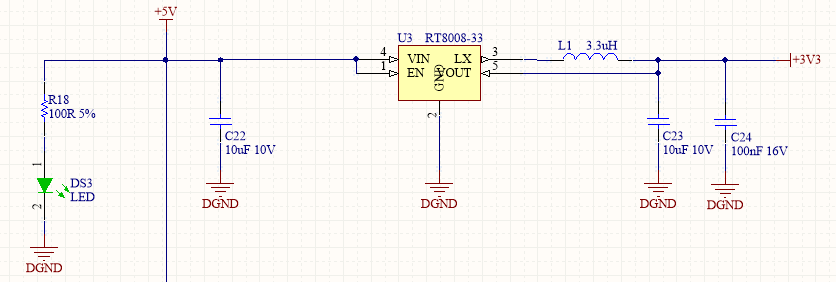
\includegraphics[width=0.8\textwidth]{power1.png}
\caption{开关电源} 
\end{figure}
数字部分采用Richtek RT8008-3.3供电。这款芯片具有以下特点:
\begin{enumerate}
\item 固定输出电压3.3V
\item 1.5MHz的PWM频率,可以使用小型的外部电感和电容
\item 内置场效应管,采用同步整流方式,具有较高的效率
\end{enumerate}\par
由于具有效率高,体积小,占用PCB面积小的特点,非常适合为本设计的数字部分供电,也利于手持设备小型化。\par
图中DS3用作电源指示灯。

\subsubsection{模拟电源}
\begin{figure}[H]
\centering
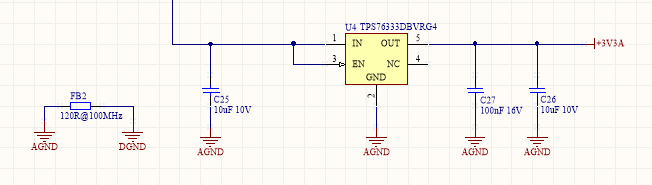
\includegraphics[width=0.8\textwidth]{power2.png}
\caption{线性电源} 
\end{figure}
模拟部分采用TI TPS79333供电。这款芯片具有以下特点:

\begin{enumerate}
\item 高PSRR(70 dB at 10 kHz)
\item 低噪声(32 $\mu V_{RMS}$)
\end{enumerate}\par
该芯片可以有效抑制电源噪声,提供符合模拟部分工作的低噪声电源。\par
图中FB2 采用120R@100MHz的磁珠将模拟地与数字地相连,可以避免数字部分对模拟部分的干扰。
\subsection{模拟前端和数据转换}
模拟前端和数据转换采用TI Audio Codec TLV320AIC23B为核心,辅以外部电路,实现声音信号和数字信号的双向转换。

\subsubsection{话筒输入}

我们采用驻极体话筒采集听诊器中的声音信号。驻极体话筒是可以看做一个已经连有输入的MOS管。
其等效电路如下:

\begin{figure}[H]
\centering
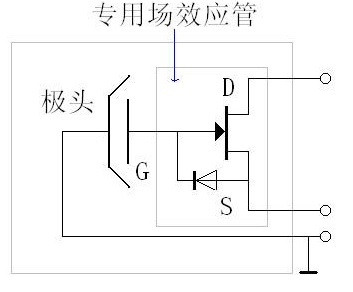
\includegraphics[scale = 0.5]{mic.jpg}
\caption{话筒等效电路} 
\end{figure}

驻极体话筒选用了松下WM62A话筒,一方面是由于其物理尺寸较小,适合放入听诊器中,另一方面是由于其在人耳可以听到的频率范围(20Hz~20kHz)中优良的频率响应特性:

\begin{figure}[H]
\centering
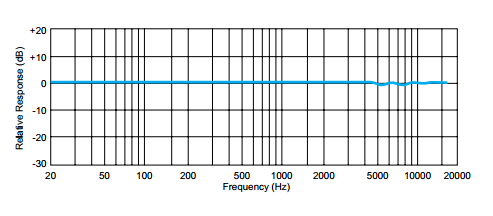
\includegraphics[scale = 1]{MICFR.png}
\caption{WM62A频率响应} 
\end{figure}

驻极体话筒的第一级放大电路是典型的共源放大电路:

\begin{figure}[H]
\centering
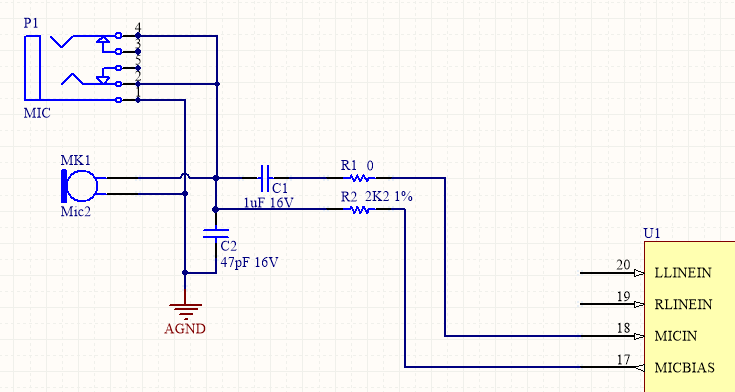
\includegraphics[scale = 0.8]{Mic2.png}
\caption{话筒输入电路} 
\end{figure}

MICBIAS为电源,它由TLV320输出,为专门用于话筒MOS管放大的低噪声偏置电压MICBIAS,可以进一步隔离电源纹波的影响。R2为共源放大电路中的$R_{s}$,通过调节R2可以调节输入信号的第一级放大增益。
输出电压经过经C1耦合后输入CODEC,下图为CODEC内部的放大电路:
\begin{figure}[H]
\centering
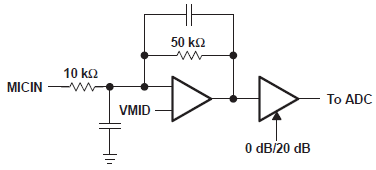
\includegraphics[scale = 1]{Mic1.png}
\caption{集成次级放大滤波电路} 
\end{figure}
第一级运放进行滤波和放大,在通带构成了一个放大倍数为5倍的放大电路,同时对20kHz以上的高频进行滤波,所以在设计时没有增加外部滤波电路。

\subsubsection{耳机输出}
\begin{figure}[H]
\centering
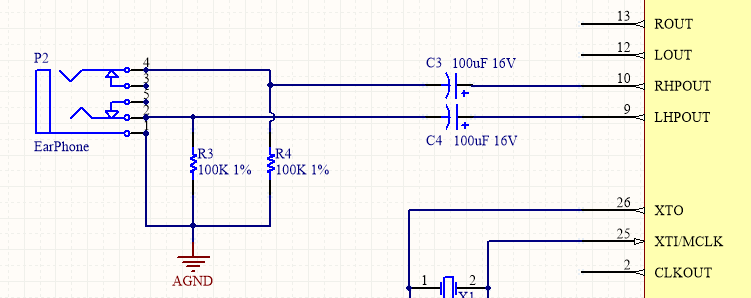
\includegraphics[width=0.8\textwidth]{EarPhone.png}
\caption{耳机输出电路} 
\end{figure}
由于芯片内置耳放,所以输出信号的左右声道分别直接通过C3和C4耦合至耳机输出即可。

\subsubsection{CODEC的数字接口}
\begin{figure}[H]
\centering
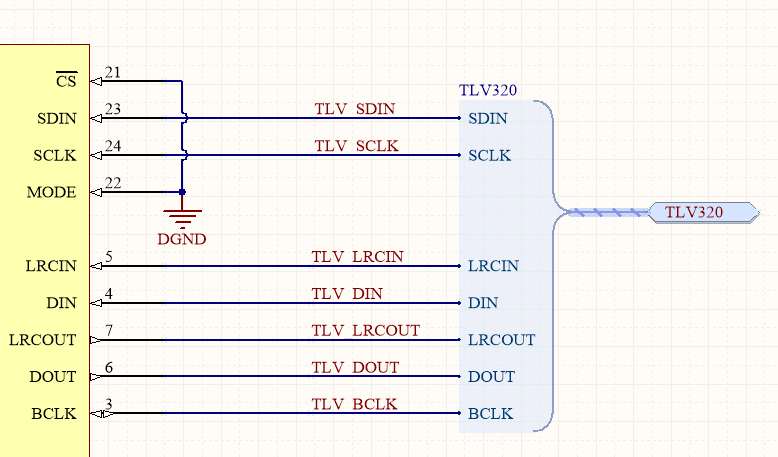
\includegraphics[width=0.8\textwidth]{DI.png}
\caption{CODEC的数字接口} 
\end{figure}
CODEC与MCU之间通过数字接口相连。控制接口为I2C接口,用于配置COEDC的输入输出方式,可编程放大器的放大增益,信号流向等。音频数据采用I2S接口相连。

\subsection{微控制器和其他数字外设}
\subsubsection{微控制器}
微控制器采用NXP LCP1768。微控制器为ARM Cortex-M3内核。
\begin{figure}[H]
\centering
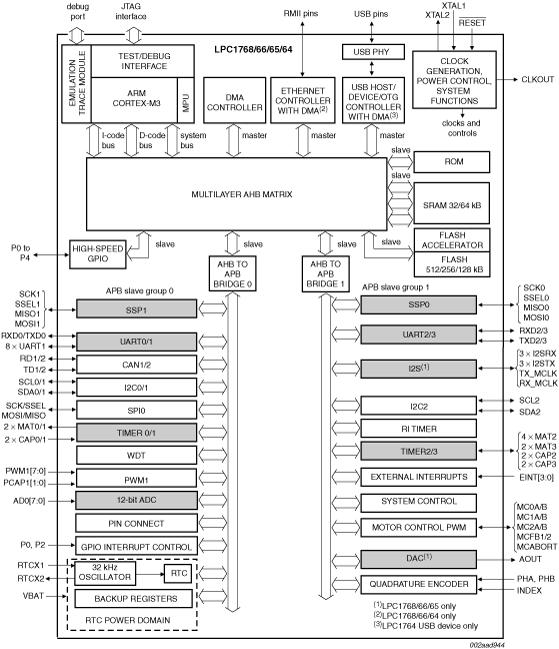
\includegraphics[width=0.7\textwidth]{LPC1768.png}
\caption{LPC1768内部框图} 
\end{figure}

\subsubsection{TF-Card}
\begin{figure}[H]
\centering
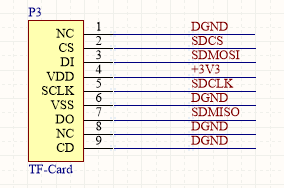
\includegraphics[scale = 0.8]{TF-Card.png}
\caption{TF-Card} 
\end{figure}

\subsubsection{USB接口}
\begin{figure}[H]
\centering
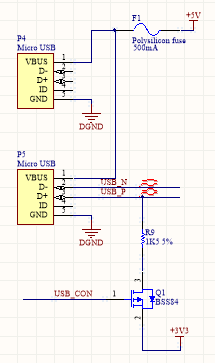
\includegraphics[scale = 1]{USB.png}
\caption{USB接口} 
\end{figure}

P4接口用于给系统供电,电源入口串有多晶硅熔丝,用于对系统和外部电源的保护。P5接口用于接驳其他的USB外部设备(如U盘)或者连接个人计算机。

\subsubsection{调试接口}
\begin{figure}[H]
\centering
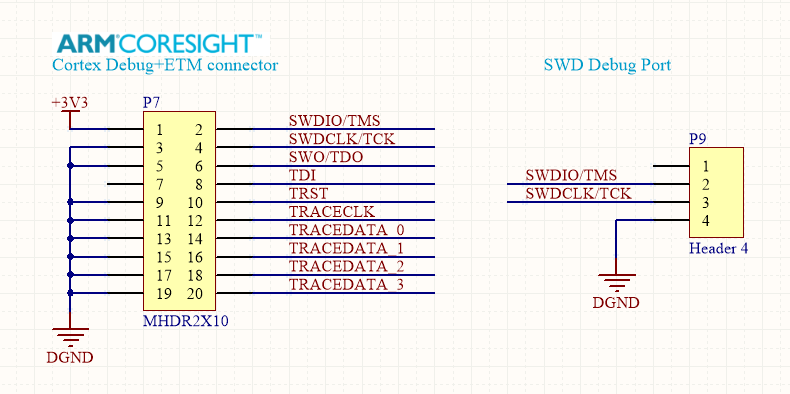
\includegraphics[width=0.6\textwidth]{debug.png}
\caption{调试接口} 
\end{figure}
留有两种调试接口。其中SWD Debug Port可以连接通用的调试工具。而标准的Cortex Debug+ETM connector可以用于连接ARM U-Link Pro等带有Trace功能的调试工具,提供更加丰富的调试功能。

\subsubsection{其他外设}
\begin{figure}[H]
\centering
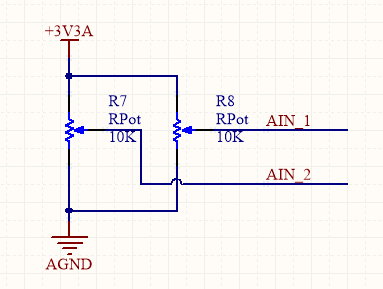
\includegraphics[scale = 0.8]{Rpot.png}
\caption{旋钮} 
\end{figure}


\begin{figure}[H]
\centering
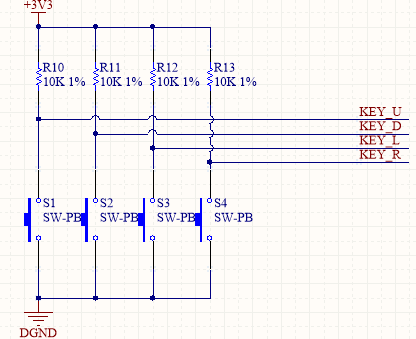
\includegraphics[scale = 0.8]{key.png}
\caption{按键} 
\end{figure}

\begin{figure}[H]
\centering
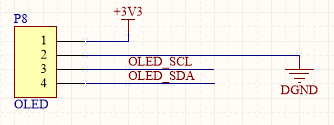
\includegraphics[scale = 0.8]{oled.png}
\caption{OLED屏幕} 
\end{figure}

这些外设可以用于扩展功能。

\section{PCB设计}
\begin{figure}[H]
\centering
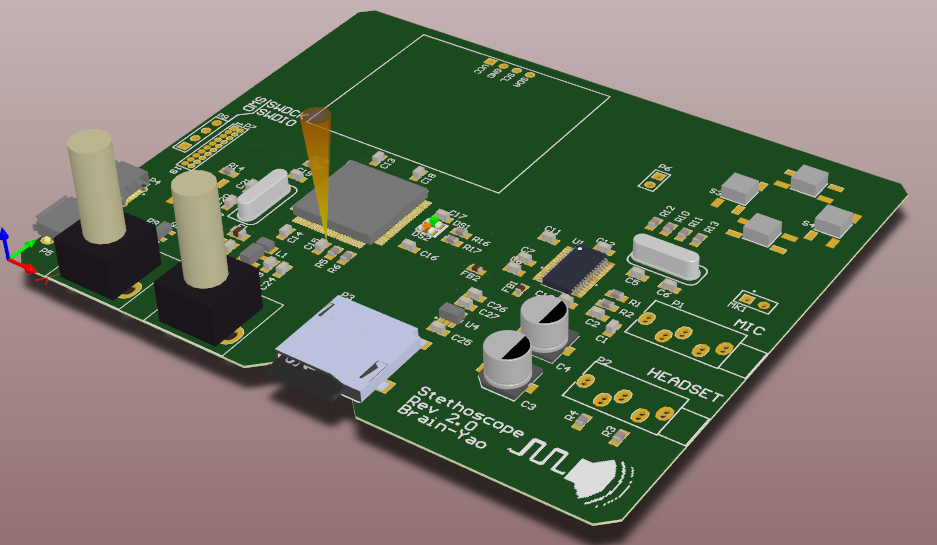
\includegraphics[width=0.8\textwidth]{pcb3D.png}
\caption{PCB三维渲染图} 
\end{figure}
PCB设计采用Altium Designer 设计,按照通常混合信号系统的设计方法,数模部分分开布局。数字地、模拟地按布局切分,单点相连。


\section{软件设计}
使用的开源库:
\begin{enumerate}
\item 软件设计中使用了ARM开发的基础库 \href{https://developer.mbed.org/users/mbed_official/code/mbed/}{mbed}。
\item 二次开发了Daniel Worrall 开发的 \href{https://developer.mbed.org/cookbook/TLV320AIC23B}{TLV320驱动库},增加了模拟输入功能以及对应的芯片配置。
\item 使用了Daniel Worrall 开发的 \href{https://developer.mbed.org/users/d_worrall/code/I2SSlave/}{I2S Slave协议库}和 Giles Barton-Owen开发的 \href{https://developer.mbed.org/users/p07gbar/code/I2S/}{I2S Master协议库}用于和CODEC芯片TLV320的通信。
\end{enumerate}


所有的代码都发布在\href{https://github.com/gjc13/Stethoscope}{开源社区github}上。

\subsection{滤波器设计}
\subsubsection{抗噪滤波器}
\begin{figure}[H]
\centering
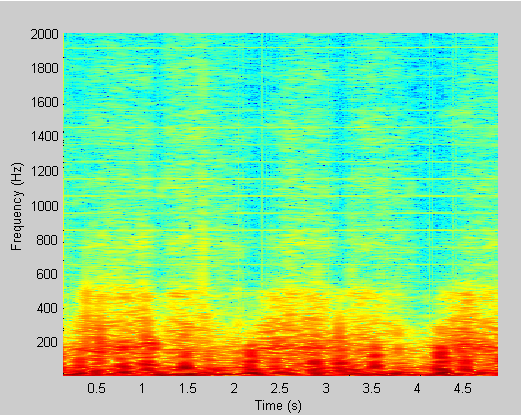
\includegraphics[scale = 1]{spectrogram_raw.png}
\caption{原始声音频谱图} 
\end{figure}
通过对采集的声音短时傅里叶变换后的频谱图的分析,主要的能量分布在1kHz以下的频段,所以使用了8kHz采样率,并且增加了一个8阶的均值滤波器用来滤去高频噪声:
\\
滤波器传递函数为:$\sum\limits_{k=0}^{7}\frac{z^{-k}}{8}$
滤波器的频率响应特性如下,截止频率大约在1100Hz左右:
\begin{figure}[H]
\centering
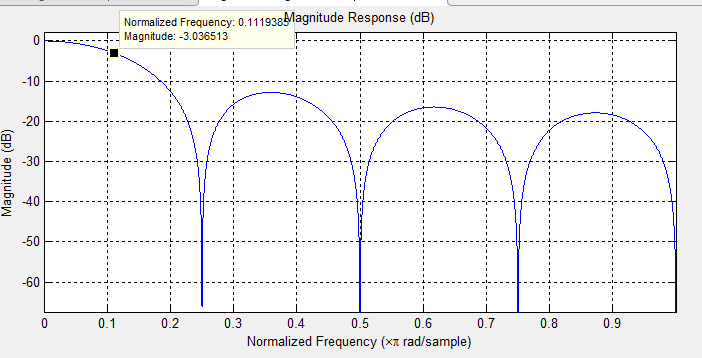
\includegraphics[scale = 0.7]{avg_filter.png}
\caption{均值滤波器} 
\end{figure}
经过滤波器滤波之后的声音信号
\begin{figure}[H]
\centering
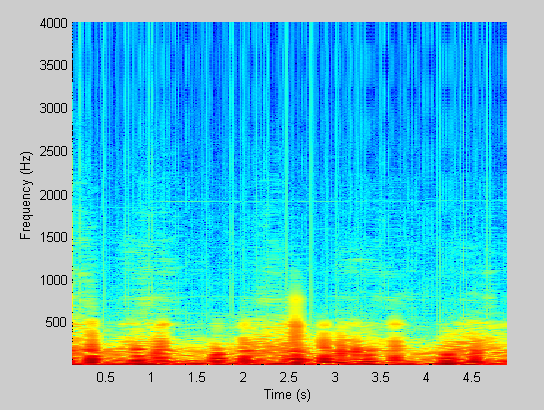
\includegraphics[scale = 1]{avg_filtered.png}
\caption{均值滤波后的声音信号} 
\end{figure} 	
\subsubsection{呼吸音加强滤波器}
由于在听诊中呼吸音往往会受到心音的干扰,所以我们考虑设计呼吸音加强的功能,由于心跳的声音频率普遍不超过500Hz,而呼吸有比较多的高次谐波,所以我们考虑使用带通滤波器加强呼吸音。但是由于呼吸音的基波频率也在500Hz以下,使用带通滤波器还是只能部分减弱心跳音。
使用的带通滤波器为64阶FIR滤波器,线性相位。频率响应如下:
\begin{figure}[H]
\centering
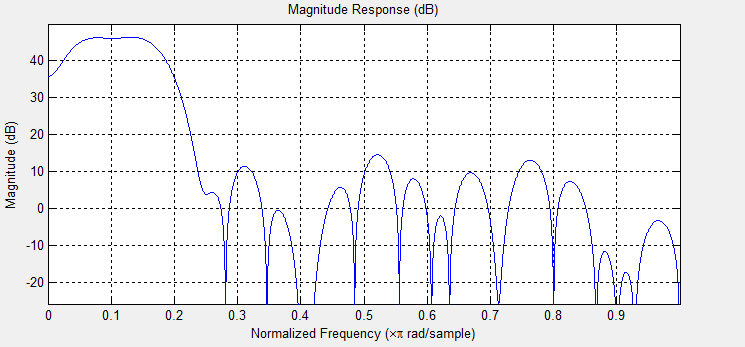
\includegraphics[scale = 0.7]{band_pass.png}
\caption{带通滤波器} 
\end{figure}
截止频率大约为400Hz和1400Hz,经过滤波后的声音信号如下:
\begin{figure}[H]
\centering
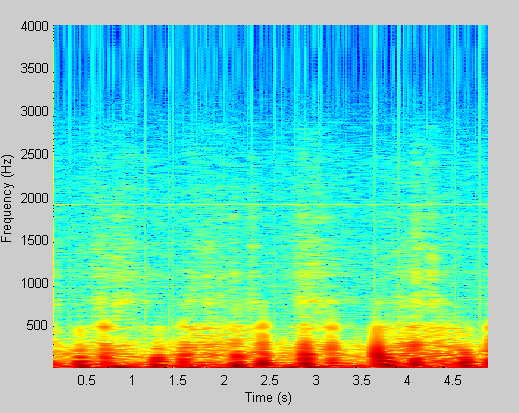
\includegraphics[scale = 1]{band_passed.png}
\caption{带通滤波后的声音信号} 
\end{figure}
实际上带通滤波并没有完全去除心跳声音而只是减弱,这一是由于呼吸音的基波和心跳音的频段有较大的重复 	,第二是由于硬件处理速度限制了滤波器的阶数使得低频段的增益不能快速下降。

\section{测试效果}
在附件中包含了录下的心跳呼吸混合声音,avgfiltered.wav是均值滤波后的效果,而bandpass.wav是呼吸音加强的带通滤波器处理的效果。由于codec已经有比较大的输出放大倍数,所以录音音量较小,在电脑上听时需要调高音量。
我们对采集到的心跳声音在电脑上使用Matlab进行分析,得到的频谱图如下:

\begin{figure}[H]
\centering
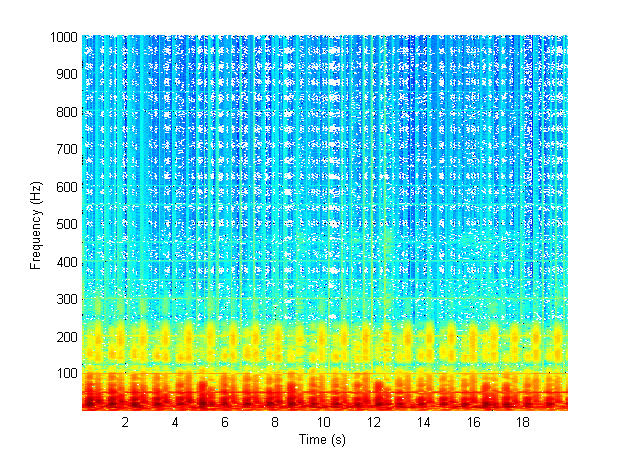
\includegraphics[scale = 0.7]{spectrogram.png}
\caption{心跳声音频谱图} 
\end{figure}
可以明显看到第一心音和第二心音的不同以及1Hz左右反复出现的心跳信号。实测发现呼吸音和心跳音在实际测试中都没有超过2kHz,所以我们考虑之后在输入级增加低通滤波电路以进一步提高信噪比。


和传统的听诊器对比,高频响应和放大倍数都有了明显提升,原来较弱的呼气音可以清晰的听到。但是信噪比不及传统听诊器,这是由于电路内部引入了不可避免的噪声,还需要进行电路设计的优化和数字滤波的处理来进一步增强信噪比。

\section{阶段总结与展望}
\subsection{取得的成果}
\begin{enumerate}
\item 设计了整体的数模混合的听诊器声音采集系统
\item 完成了所有的芯片的软硬件调试工作
\item 进行了初步的信号采集与分析
\item 设计了不同的滤波器用于滤波和特定频段放大
\end{enumerate}
\subsection{阶段感受}
在信号课程设计的过程中,我们完成了一个完整的信号处理系统的软硬件设计。其中尤其大的感受是信号处理是需要各个方面大量的软硬件技术配合才能达到比较好的效果。比如在我们的调试过程中,初期噪声总是非常大,如果使用低通滤波器尽心降噪需要将截止频率降到200Hz左右,呼吸音几乎一斤完全听不到。但是通过对硬件的调试,发现sd卡槽的金属盖没有接地,将其接地后立刻就大大降低了噪声。同时许多软件算法也会受到硬件的限制,NXP1768处理器的处理能力以及RAM大小都限制了我们不能使用很高阶的滤波器以及处理必须是实时的,不可能进行存储后再处理,也对软件设计提出了很多挑战,同时影响了一些最终滤波的效果。
\subsection{之后的工作与展望}
\begin{enumerate}
\item 根据听诊器声音信号的特点,在前级进一步添加截止频率在2kHz左右的低通滤波电路以减小噪声。
\item 进一步开发心跳检测呼吸检测等功能。
\end{enumerate}

\end{document}
